\chapter{Transcrire les données des factures Rondel dans la base \emph{Heurist} : modélisation et premiers essais d'implémentation} 

La modélisation de la base de données s'est rapidement suivie de sa conception dans \emph{Heurist}\index{Heurist}, par la création des \emph{Record types} et des principaux champs de cette base, dont l'objectif principal est la transcription des données depuis les factures Rondel, qu'il faut garder à l'esprit comme étant le fil directeur de tout ce travail.
Il convient donc de présenter dans ce chapitre la majeure partie des champs, spécialement prévus pour accueillir les informations issues des factures. Cette présentation s'accompagnera de considérations liées à la saisie de ces informations dans la base, ainsi qu'aux limites d'Heurist constatées au cours de ce travail. 

\section{Conception d'une base \emph{Heurist}\index{Heurist} à partir des informations issues des factures Rondel : \emph{Record types}, \emph{fields} et vocabulaires contrôlés} 
\label{conception base}


Comme nous pouvons le lire sur le modèle de données, la base de données est composée de cinq \emph{Record types}, ou cinq tables, chacun se concentrant sur l'un des aspects, précédemment évoqués, que nous avons relevés en analysant les factures Rondel, à savoir les lieux où Rondel se fournit, les personnes mentionnées, les factures, et les titres achetés. 
La constitution de ces \emph{Record types} entend affiner notre analyse de ces différents aspects, tout en les adaptant à la forme d'une base \emph{Heurist}. 

À ce titre, les données concernant les librairies sont scindées en deux \emph{Record types}. Le premier, nommé \enquote{librairie}, sert à renseigner des informations concernant les établissements, à savoir leur nom et leur spécialité. il est également possible de lier deux enregistrements \enquote{librairie} entre eux grâce à une relation (de type \emph{Relationship marker}) nommée \enquote{succursale}. Cette relation sert à indiquer les liens entre des librairies et leur succursale, que l'on a considéré comme des établissements à part entière. Grâce à un vocabulaire contrôlé appelé \enquote{RelationsLibrairies}, ce champ permet d'indiquer qu'une librairie est la succursale d'une autre. Cette relation est réciproque : la relation \enquote{EstSuccursaleDe} génère automatiquement une relation inverse \enquote{APourSuccursale}. 

\begin{figure}[htbp]
    \centering
   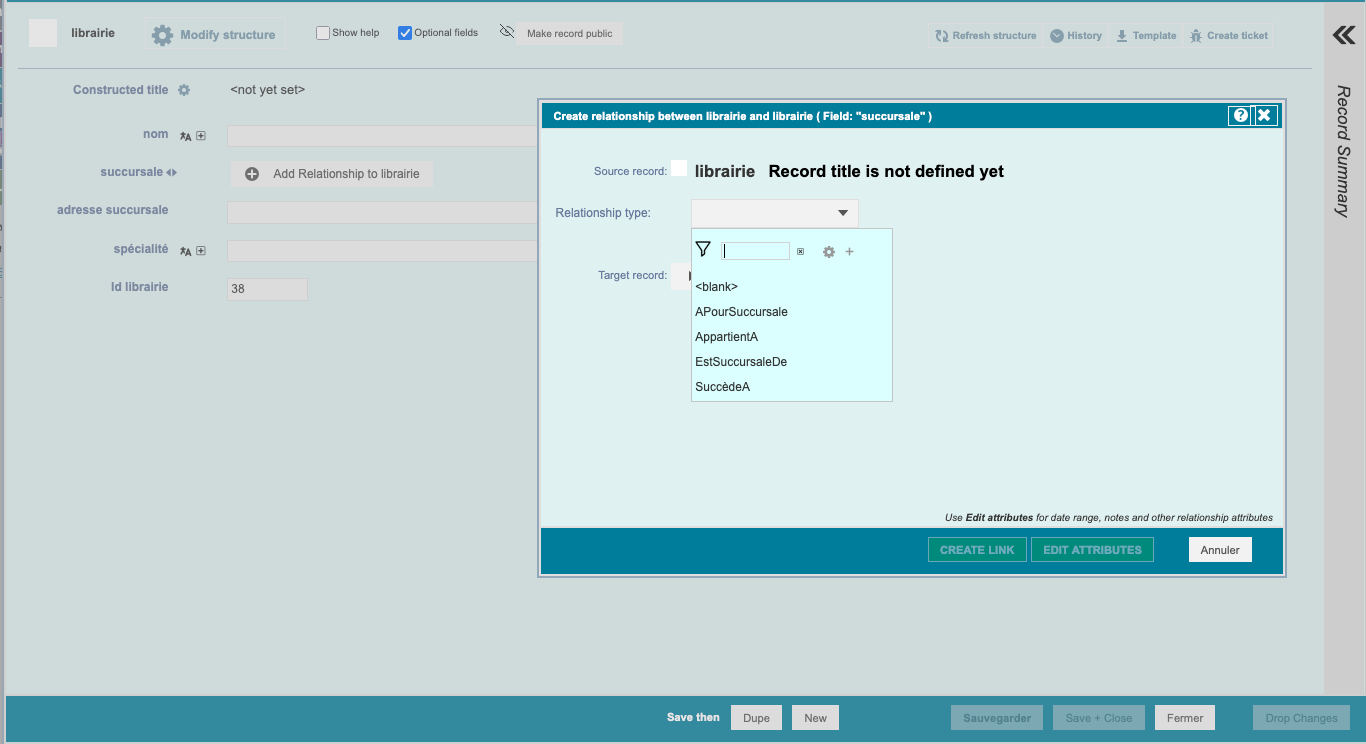
\includegraphics[width = 15cm]{Images/librairiesuccursale.png}
    \caption{Champ \enquote{succursale} dans le \emph{Record type} \enquote{librairie}. }
    \label{fig:champ-succursale}
\end{figure}

Le deuxième, appelé \enquote{lieu}, sert à distinguer les différents lieux occupés par les librairies. Il est surtout utile en cas de déménagement d'une librairie, phénomène fréquemment relevé dans les factures Rondel. 
L'intérêt est de pouvoir dater l'appartenance d'un lieu à un établissement grâce au champ \enquote{librairie}. Toujours grâce au vocabulaire contrôlé \enquote{RelationsLibrairies}, ce champ nous permet de lier notre enregistrement \enquote{lieu} à un enregistrement \enquote{librairie} pour une période donnée, grâce au terme \enquote{AppartientA}, et en soumettant cette relation d'appartenance à des bornes chronologiques, ce qui est l'un des intérêts des \emph{Relationship markers}. 

\begin{figure}[htbp]
    \centering
   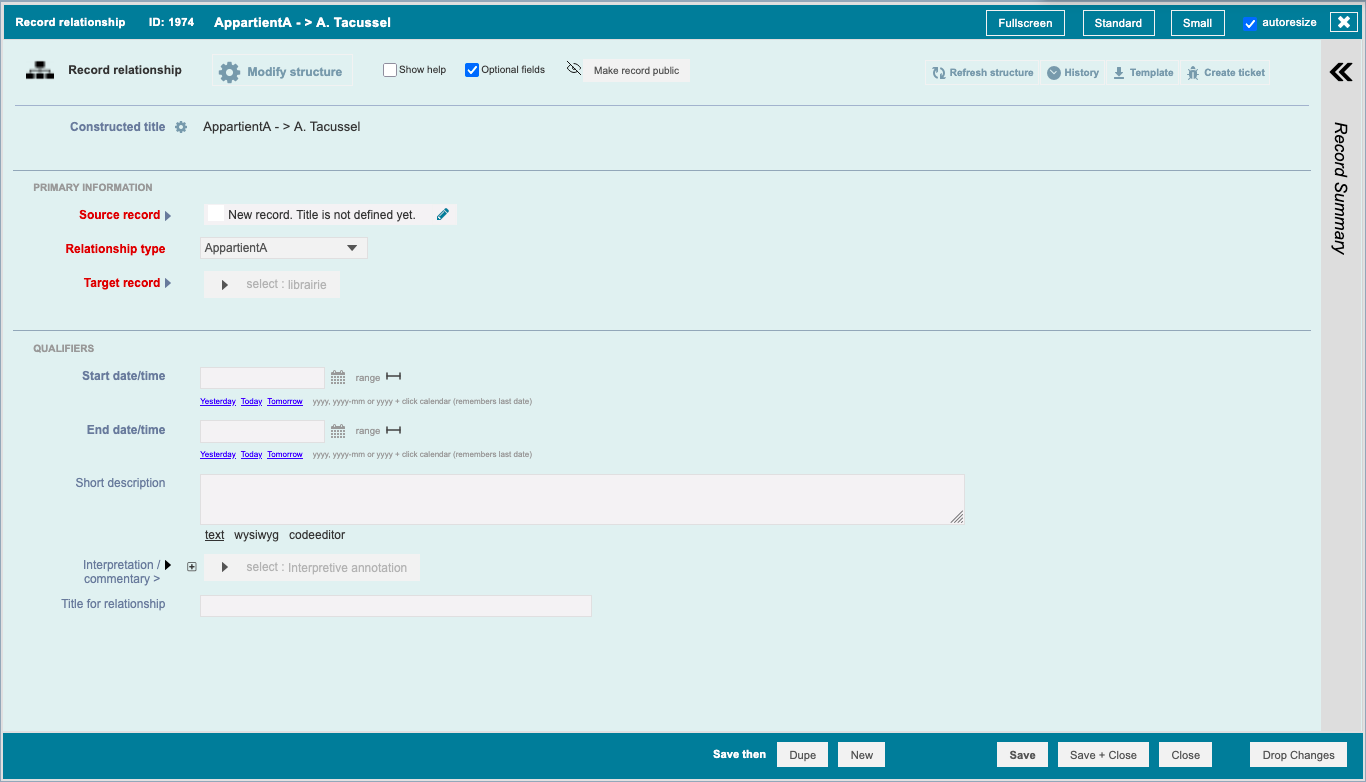
\includegraphics[width=15cm]{Images/Lieu.png}
    \caption{Remplissage du champ \enquote{librairie} de la table \enquote{lieu}.}
    \label{fig:champ-lieu-librairie}
\end{figure}

Les autres champs de ce \emph{Record type} permettent de situer les lieux spatialement. En voici deux exemples : 

Les champs \enquote{ville} et \enquote{pays}, sont tous les deux des choix déroulants parmi des vocabulaires contrôlés, constitués de listes de tous les pays et villes rencontrés dans les factures Rondel. Ces listes de lieux ne sont pas exhaustives, et seront amenées à être enrichies par les nouvelles villes et les nouveaux pays rencontrés dans le reste du corpus. 


Comme prévu, un \emph{Record type} de cette base, appelé \enquote{personne}, est avant tout conçu pour transcrire les informations concernant des personnes et issues des factures.
La plupart des champs servent à accueillir des informations assez sommaires trouvables dans les factures, telles que leurs noms, prénoms et professions (libraires le plus souvent). Grâce à un lien de type \emph{Record pointer}, chaque personne recensée est liée à l'établissement où elle travaille. Un champ de ce \emph{Record type}, appelé \enquote{PersonneAssociée}, permet d'indiquer des liens de différentes natures entre les personnes. Ce champ s'appuie encore sur un vocabulaire contrôlé, nommé \enquote{LiensEntrePersonnes}, et réalisé à partir des liens interpersonnels observés dans les factures. Ce vocabulaire définit d'abord le lien le plus évident que l'on peut percevoir dans les factures : les liens professionnels entre les personnes. 

\begin{figure}[htbp]
    \centering
    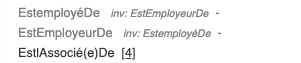
\includegraphics[width=10cm]{Images/LiensPro.png}
    \caption{Exemple de vocabulaire consacré aux liens professionnels entre les personnes}
    \label{fig:liens-professionnels}
\end{figure}

L'image ci-dessus montre les deux types de liens professionnels que nous avons modélisés : un lien \enquote{EstEmployeurDe}, lui aussi réciproque, dont le lien inverse est \enquote{EstEmployéDe}, et un lien plus simple, utilisé lorsque deux personnes travaillent ensemble sans lien de subordination visible, appelé \enquote{EstAssocié(e)De}. 

Les établissements étant souvent tenus par des familles de libraires, nous avons également décrit avec précision les différents types de liens familiaux susceptibles d'apparaître dans les factures. Pour ce faire, nous nous sommes inspirés d'un vocabulaire contrôlé déjà existant dans \emph{Heurist}\index{Heurist}, le vocabulaire \enquote{Family}, issu du groupe \enquote{Relationships}, qui représente tous les types de relations familiales pouvant exister. 

\begin{figure}[htbp]
    \centering
    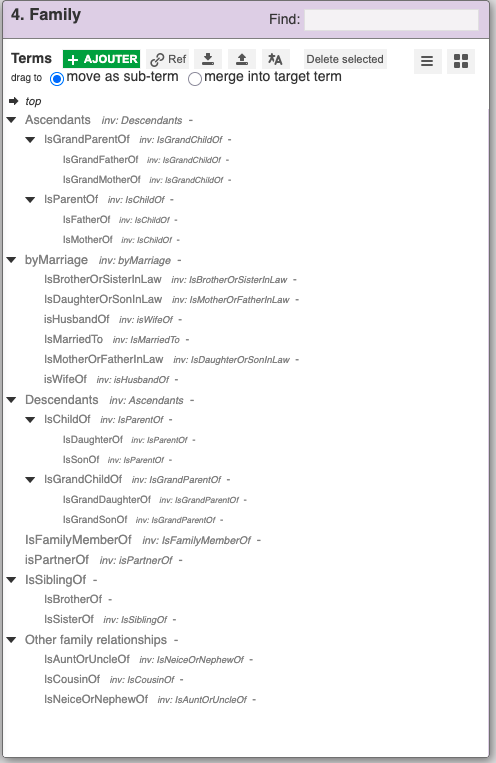
\includegraphics[width=7cm]{Images/family.png}
    \caption{Vocabulaire \enquote{Family}}
    \label{fig:vocabulaire-family}
\end{figure}
  
\begin{figure}[htbp]
    \centering
    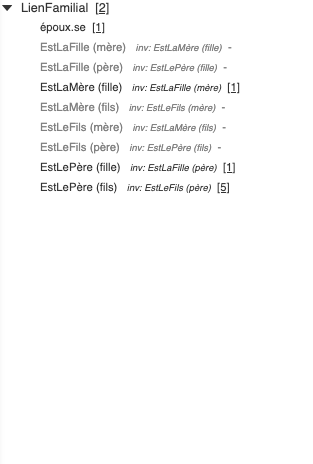
\includegraphics[width=7cm]{Images/LiensFamiliaux.png}
    \caption{Liens familiaux}
    \label{fig:liens-familiaux}
\end{figure}


\vspace{1.5cm}

Dans notre base de données, nous avons également représenté des liens réciproques, et en étant le plus précis possible, comme le montre l'image ci-dessous. 

\newpage
Le \emph{Record type} le plus important de cette base, et qui a vocation a être le plus fourni est sans aucun doute \enquote{ligne de facture}, ayant pour but de recenser chaque titre acheté par Rondel auprès d'une librairie. Cette table vise à répondre à l'un des objectifs principaux de ce travail, à savoir de retracer la provenance des oeuvres de la collection Rondel. Une partie des champs de cette table, spécialement dédiée à la transcription des factures, prévoit donc la possibilité de saisir tous types d'informations que nous avons relevées dans ces lignes, et qui concernent les oeuvres achetées. 

\begin{figure}[htbp]
    \centering
    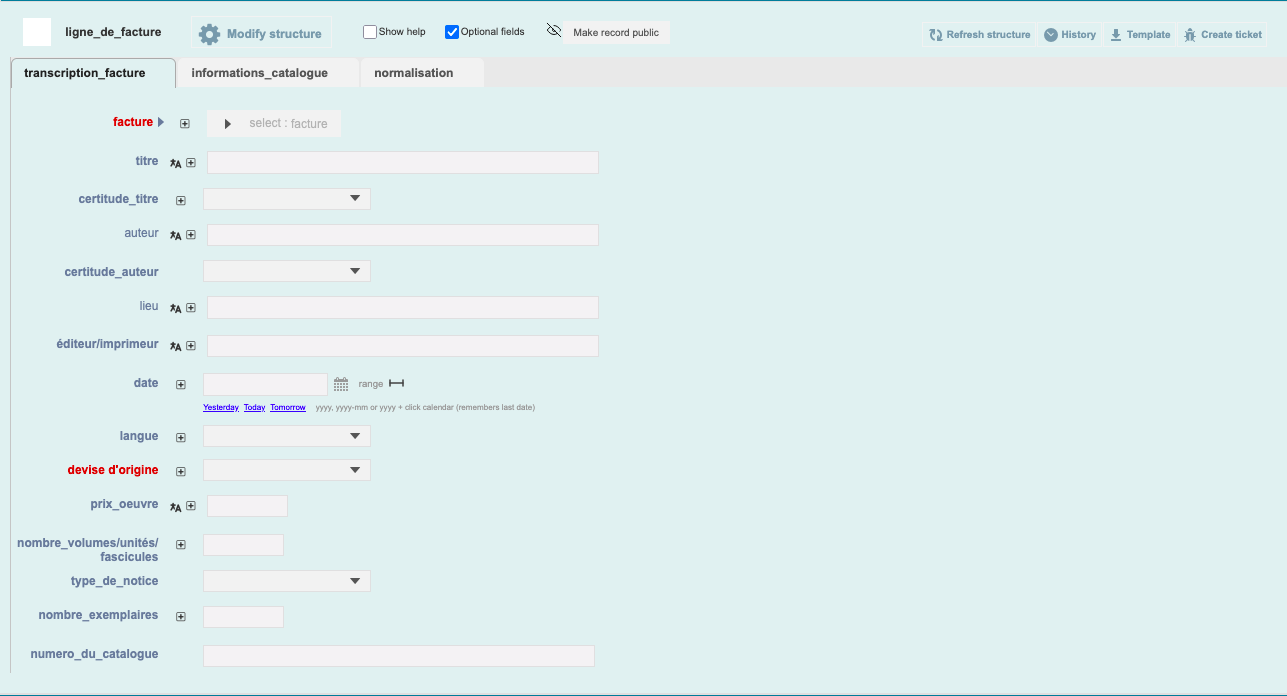
\includegraphics[width=12cm, height=8cm]{Images/transcription ligne facture.png}
    \caption{Champs de la table \enquote{ligne de facture} prévus pour les informations directement transcrites des factures.}
    \label{fig:champs-ligne-facture}
\end{figure}

Comme on peut le constater sur le formulaire de saisie ci-dessous, les champs concernent des informations variées, allant du plus évident et indispensable pour retrouver une oeuvre (titre, auteur, date, ...) à des informations plus précises, que l'on ne peut trouver que dans certaines factures (éditeur/imprimeur, lieu, ou encore le numéro qui identifie l'oeuvre dans les catalogues des libraires, ...). Peuvent aussi être renseignés les prix des oeuvres et leurs devises, qui encore une fois font l'objet d'un vocabulaire contrôlé. 
On peut voir que les champs obligatoires de cette table (en rouge) sont très rares, comparés aux champs dits \enquote{recommandés}, qui sont majoritaires. Nous avons fait ce choix car le niveau d'information dans les factures est, nous l'avons dit, très hétérogène. Le but est que le manque de données sur la facture ne devienne jamais un obstacle pour en saisir les informations dans la base.  

\vspace{1.5cm}
Afin de pouvoir remonter à la source des informations, chaque enregistrement \enquote{ligne de facture} est lié à un  autre enregistrement, saisi au préalable, de type \enquote{facture}. Il s'agit du cinquième et dernier \emph{Record type} qui compose cette base, et son rôle est d'indexer chaque facture, et de renseigner les informations principales la concernant, et utiles pour la retrouver. On trouve donc l'établissement producteur de la facture ainsi que sa date, mais aussi la cote du dossier où elle est rangée, ce qui n'est pas forcément indispensable car, nous l'avons vu, chaque dossier est en général consacré à un libraire, mais peut toujours être utile dans certains cas. Au-delà de ces informations essentielles, cette table recense aussi toutes les données qui concernent directement la facture, à savoir le nombre de titres qui la compose, son montant et les frais souvent inclus  (frais de port, ...), ou encore la devise dans laquelle le paiement est fait (reposant sur le même vocabulaire contrôlé que pour la table précédente).

Ces deux dernières tables correspondent donc à deux échelles d'information venant des factures : l'une à une échelle très large, celle des factures, relevant plutôt de l'analyse du document en lui-même et de sa structure, et l'autre à l'échelle de la ligne de facture qui, beaucoup plus précise, répond directement à l'objectif d'identification des titres achetés. 


\newpage

\section{La saisie de données}

La saisie manuelle de données est une pratique nécessaire à l'enrichissement et à l'évolution de cette base de données. Elle demeure en effet le moyen privilégié pour transcrire les données des factures à la base. Plus qu'un moyen, la saisie est également la meilleure façon de connaître intimiment les sources sur lesquelles on travaille, et suscite inévitablement des nouveaux questionnements\footcite{Lemercier_Zalc_2008}. L'étape de saisie de données est donc essentielle, car elle permet d'éprouver le modèle que nous avons conçu, et de le faire évoluer en fonction de ce qu'on rencontre dans les sources, dans le but, à terme, de le stabiliser. 
La saisie au sein de cette base a été pensée selon des bonnes pratiques à respecter\footcite[Voir les dix commandements  de la saisie]{Lemercier_Zalc_2008}. Nous avons par exemple accordé une attention particulière au fait de conserver avec précision l'orthographe de la source, et de ne l'avoir modernisée qu'\emph{a posteriori}, dans des champs spécifiques de la base. Les informations ajoutées, extérieures à la source, sont donc  séparées nettement de celles issues des factures. 
L'étape de saisie pourra être réalisée par des conservateurs, des chercheurs, et quiconque utilisera la base. Pour cela, une documentation détaillant tous les usages ultérieurs possibles de la base, et destinée aux futurs utilisateurs explique entre autres, champ par champ, comment saisir manuellement les informations dans la base\footnote{Un renvoi vers cette annexe sera fait ici quand celle-ci sera finalisée}. 

Ainsi, la saisie de données est la façon la plus évidente d'envisager le traitement informatique de ce corpus, mais aussi d'enrichir la réflexion sur ce que peuvent nous dire ces factures. Cette pratique doit donc être particulièrement fléchée et encadrée. 


\section{Limites d'\emph{Heurist}}


Les objectifs et la portée de ce projet doivent aussi être définis en gardant en tête qu'Heurist est limité sur de nombreux aspects. 
Les limites d'\emph{Heurist}\index{Heurist} concernent à la fois son fonctionnement général et certains aspects techniques plus précis. 

De manière générale, le principal défaut d'\emph{Heurist}\index{Heurist} est le manque de documentation à son sujet, et le fait que la documentation ne soit pas assez actualisée. Il existe une documentation officielle en anglais sur \emph{Heurist}, mais celle-ci peut être difficile à appréhender\footcite{heurist_help}. La documentation française, quant à elle, est très dispersée, et se présente sous la forme de tutoriels réalisés par différentes institutions, comme par exemple Huma-Num, qui héberge le logiciel\footcite{huma-num_heurist_2026}. Une autre difficulté liée à cette documentation est que le logiciel est régulièrement actualisé, et que la documentation ne l'est pas systématiquement. Par conséquent, elle ne correspond pas toujours à ce que l'on trouve actuellement dans le logiciel, ce qui peut être déroutant. Pour compenser cela, la liste de diffusion officielle gérée par la communauté d'utilisateurs, très active, d'\emph{Heurist}, nous a permis de nous tenir au courant de l'actualité du logiciel et même à poser des questions en cas de difficulté\footcite{noauthor_heurist-utilisateurs_nodate}. 

La forme d'\emph{Heurist}\index{Heurist} fait que nous avons également été limités dans nos possibilités techniques, c'est pourquoi nous avons dû utiliser des moyens détournés pour parvenir à mettre en oeuvres certaines fonctionnalités de notre base de données. Par exemple, Heurist\index{Heurist} n'a pas un type de données spécialement dédié aux booléens, c'est-à-dire aux réponses par \enquote{oui} ou par \enquote{non}. Ce type de données est pourtant assez classique, et très courant dans les jeux et les bases de données. \emph{Heurist}\index{Heurist} prévoit malgré tout l'utilisation de ce type de données de manière détournée. En effet, certains vocabulaires contrôlés qui pré-existaient à notre base jouent le rôle des booléens. C'est le cas, au sein du groupe de vocabulaires \enquote{Categorisation and flags}, de deux vocabulaires nommés \enquote{Flag}, dont l'un contient \enquote{Yes} et \enquote{No}, et l'autre \enquote{Yes}, \enquote{No} et \enquote{Unknown}. Ils peuvent donc être utilisés comme des vocabulaires contrôlés classiques, et exprimer un choix entre oui et non. Il faut noter qu'il est tout à fait possible de créer son propre vocabulaire contrôlé composé des options \enquote{oui} et \enquote{non}, dans n'importe quelle langue. 
Le fait de pouvoir choisir des niveaux de certitude des informations pour les données en format \enquote{date} a été beaucoup apprécié dans l'utilisation du logiciel. Cependant, il aurait été plus adapté aux objectifs de notre projet que cette option n'existe pas que pour les dates, et soit disponible pour d'autres types de données. En effet, nous étions obligés de rentrer des informations hypothétiques dans la base lorsque nous n'étions pas sûr de l'orthographe d'un mot où de l'exactitude d'un intitulé écrit sur une facture. Pour pallier à cela, nous avons créé des champs dédiés pour les informations essentielles de la base : des champs \enquote{certitude titre} et \enquote{certitude auteur}, constitués des options \enquote{oui} et \enquote{non}. 

\vspace{1.5cm}

Ainsi peut-on résumer l'exploitation d'un maximum de données des factures Rondel et leur retranscription dans la base \emph{Heurist}\index{Heurist}. Il convient maintenant de s'intéresser à tous les traitements que ce logiciel nous permet de réaliser à partir de ces données, qu'il s'agisse d'enrichissements ou de visualisations. 